\frame{
	\frametitle{Blocking}

		\begin{columns}
		\column{.6\textwidth}
			\begin{itemize}\itemsep=20pt
				\item Grouping traversals in blocks allows locality improvements for deeper structures;

				\item All block elements must follow similar path (achieved with Spatial Sort);
			\end{itemize}
		
			\begin{figure}
				\centering
				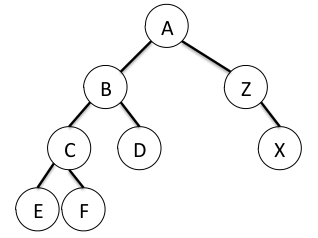
\includegraphics[width=0.5\columnwidth]{pointblocking_tree}
			\end{figure}

		\column{0.4\textwidth}

			\begin{figure}
				\centering
				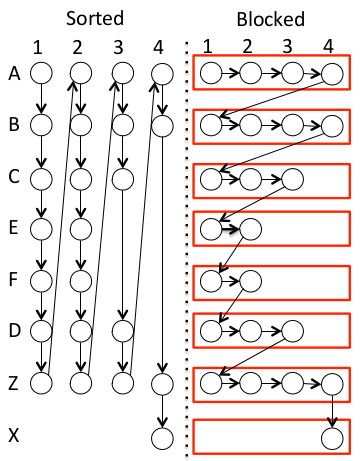
\includegraphics[width=0.9\columnwidth]{pointblocking_blocks}
			\end{figure}
	\end{columns}
}